\documentclass[10pt,aspectratio=169]{beamer}

\usepackage[american]{babel}

\usetheme[sectionpages]{sesalcf}
\sesalcflight % white content slides
\usepackage{appendixnumberbeamer}
\usepackage{ulem}
\usepackage[newfloat]{minted}
\usepackage{booktabs}
\usepackage{csquotes}
\usepackage{array}
\usepackage{tikz}
\usetikzlibrary{positioning,arrows.meta}

\setminted[bash]{xleftmargin=\parindent,fontsize=\scriptsize,baselinestretch=1,breaklines}
\setminted[text]{xleftmargin=\parindent,fontsize=\scriptsize,baselinestretch=1,breaklines}
\setminted[c++]{xleftmargin=\parindent,fontsize=\scriptsize,baselinestretch=1, breaklines}
\setminted[c]{xleftmargin=\parindent,fontsize=\scriptsize,baselinestretch=1, breaklines}
\setminted[python]{xleftmargin=\parindent,fontsize=\scriptsize,baselinestretch=1, breaklines}
\setminted[json]{xleftmargin=\parindent,fontsize=\scriptsize,baselinestretch=1,breaklines}
\setminted[toml]{xleftmargin=\parindent,fontsize=\scriptsize,baselinestretch=1,breaklines}
\setminted{bgcolor=SESpanelLight}

\providecommand{\tightlist}{%
  \setlength{\itemsep}{0pt}\setlength{\parskip}{0pt}}

\title{Vibecoding With ALCF Inference}
\subtitle{Programming with open-weight models on ALCF hardware}

\date{\today}
\author{Ethan Wong}

\begin{document}

\begin{frame}[plain]
\maketitle
\end{frame}

\section{Introduction}

\begin{frame}{What is Vibecoding?}
  \begin{itemize}
    \item Term coined by Andrej Karpathy (Feb 2025):
    \begin{quote}\small\itshape
      \enquote{There's a new kind of coding I call \enquote*{vibe coding},
	    where you fully \\ give in to the vibes, embrace exponentials and
	    forget that the code even exists.}
    \end{quote}
    \item \textbf{In practice:} you describe what you want in plain language
	    and a \emph{coding agent} writes, runs, and debugs the code. You
		  iterate by \emph{reviewing the results} and
		  \emph{re-prompting} instead hand-writing code.
    \item Note that this doesn't absolve critical-thinking! You still need to
	    do the hard work of discerning \emph{what} to make, how
		  \emph{robust} it's built, and judging whether it is
		  \emph{correct}.
    \item For domain scientists: the barrier shifts from syntax and
	    software-development expertise to specification and verification,
		  skills you already have.
  \end{itemize}
\end{frame}

\begin{frame}{From Chatbots to Coding Agents}
  \begin{itemize}
    \item \textbf{2021--22:} IDE autocomplete brings Copilot
      suggestions into your editor, still line-by-line
    \item \textbf{2022:} Chat assistants. You copy/paste snippets from
      the chat window, run everything, and fix every error
    \item \textbf{2024--25:} Terminal \emph{agents} that read/write files,
      run shell commands, search the repo, observe errors, and self-correct
  \end{itemize}
  \vspace{0.5em}
  \centering
  \begin{tikzpicture}[node distance=0.75cm,
      every node/.style={font=\scriptsize, text=SESink},
      flowbox/.style={draw=SESteal, fill=SESpanelLight, rounded corners, inner sep=4pt}]
    \node[flowbox] (prompt) {prompt / intent};
    \node[flowbox, right=of prompt] (plan) {plan};
    \node[flowbox, right=of plan] (act) {act (tools)};
    \node[flowbox, right=of act] (observe) {observe};
    \node[flowbox, right=of observe] (done) {done};
    \draw[-stealth, draw=SESteal] (prompt) -- (plan);
    \draw[-stealth, draw=SESteal] (plan) -- (act);
    \draw[-stealth, draw=SESteal] (act) -- (observe);
    \draw[-stealth, draw=SESteal] (observe) -- (done);
    \draw[-stealth, draw=SESteal] (observe) to[bend right=45]
      node[below, font=\scriptsize, text=SESgrey] {errors? refine and retry} (plan);
  \end{tikzpicture}\par
  \vspace{0.5em}
  \raggedright
  The agent is now the \emph{executor}. You now focus on the overall
	architecture and review.
\end{frame}

\begin{frame}{Anatomy of a Coding Agent}
  \begin{itemize}
    \item An \textbf{agent harness} is this read-eval-print loop as one
      coherent piece of software\footnote{Exactly what you built in the
      previous session!} with:
    \begin{itemize}
      \item \textbf{Tools:} read/edit/write files, run shell commands, search
        the codebase, (sometimes) the web
      \item \textbf{Loop:} model proposes action $\rightarrow$ tool executes
        $\rightarrow$ output observed $\rightarrow$ repeat until done
      \item \textbf{Guardrails:} approval prompts, sandboxing, git
    \end{itemize}
    \item Example popular harnesses. All support \emph{external providers}, so
      they can point at ALCF Inference:
    \begin{itemize}
      \item \textbf{OpenCode} (what we'll demonstrate this session) and
	      \textbf{Pi}, recommended in the ALCF docs
      \item \textbf{Claude Code}, featured in the session right after
        this one
      \item \textbf{Codex}, OpenAI's in-house harness for their GPT model series
      \item Additionally, there are community shims/proxies for anything else
	      (see \texttt{alcf-proxy}, \texttt{llm-rosetta})
    \end{itemize}
  \end{itemize}
\end{frame}

\section{The ALCF Inference Service}

\begin{frame}{ALCF Inference Endpoints at a Glance}
  \begin{itemize}
    \item \textbf{30+ open-weight models} on ALCF hardware,
      behind one OpenAI-compatible API
    \item The ALCF Inference Service is accessible with \emph{any} DOE lab
	    credentials via Globus; today you should authenticate using your
		  \textbf{ALCF} login.
    \item Web UI: \url{https://inference.alcf.anl.gov}, or query the API
      directly
    \item Billions of LLM tokens for agents already served
  \end{itemize}
  \vspace{0.5em}
  \begin{table}
    \centering\footnotesize
    \begin{tabular}{@{}lll>{\raggedright\arraybackslash}p{4.1cm}@{}}
      \toprule
      Cluster & Hardware & Base path & Wire APIs \\
      \midrule
      Sophia & NVIDIA A100 & \texttt{/resource\_server/sophia/vllm/v1} & chat, responses\footnotemark, messages\footnotemark[1], completions, embeddings \\
      Metis & SambaNova SN40L & \texttt{/resource\_server/metis/api/v1} & chat, responses\footnotemark[1] \\
      Minerva & NVIDIA B200 & \texttt{/resource\_server/minerva/api/v1} & chat, responses, messages, completions, embeddings \\
      \bottomrule
    \end{tabular}
  \end{table}
  \footnotetext{Streaming for these APIs is disabled on Sophia and
    Metis, use Chat Completions or Minerva instead}
\end{frame}

\begin{frame}{Picking a Model for Agents}
  \begin{itemize}
    \item Agents \emph{talk} to models through \textbf{tool calling}; the
      harness advertises tools (read file, run command, \dots) and the model
      replies with structured calls
    \item Capability flags in the docs: \textbf{B}atch, \textbf{R}easoning,
      \textbf{T}ool calling, always \textbf{H}ot
    \item Agents need models with \textbf{T}; \textbf{R} improves planning;
      \textbf{H} avoids cold starts
  \end{itemize}
  \vspace{0.5em}
  \setcounter{footnote}{0}
  \begin{table}
    \centering\footnotesize
    \begin{tabular}{@{}llll>{\raggedright\arraybackslash}p{4.6cm}@{}}
      \toprule
      Model (subset) & Cluster & Flags & Score\footnote{Artificial Analysis
        Intelligence Index v4.3.2 (current), each model at its best
        reasoning effort.} & Notes \\
      \midrule
      \textbf{\texttt{inkling-bf16}} & Minerva & RTH & 25 & 975B MoE; recommended \\
      \texttt{nemotron-3-ultra} & Minerva & RTH & 23 & 550B MoE, 1M context; near-tie \\
      \texttt{openai/gpt-oss-120b} & Sophia & BRTH & 12 & batch + always hot; safe default \\
      \texttt{gpt-oss-120b} & Minerva & RT & 12 & same model; not live on Minerva \\
      \bottomrule
    \end{tabular}
  \end{table}
\end{frame}

\section{Setting Up Your Harness}

\begin{frame}[fragile]{Install the Agent}
  \begin{minted}[fontsize=\footnotesize]{bash}
# OpenCode
curl -fsSL https://opencode.ai/install | bash

# Claude Code (next session!)
curl -fsSL https://claude.ai/install.sh | bash

# reload your shell afterwards (zsh: ~/.zshrc, or open a new terminal)
source ~/.bashrc
  \end{minted}
  \begin{itemize}
    \item These one-liners install to \texttt{\textasciitilde/.local/bin}.
    \item Also available via \texttt{brew}, \texttt{apt}, etc.\footnote{See the
      \texttt{\#agents} section of the ALCF Inference docs for other agents}
  \end{itemize}
\end{frame}

\begin{frame}[fragile]{Quick Configuration: \texttt{alcf-ai}}
  \begin{itemize}
    \item \texttt{alcf-ai} writes generates a provider config that
      \textbf{refreshes your access token automatically}
  \end{itemize}
  \begin{minted}[fontsize=\footnotesize]{bash}
# install uv if you don't have it
curl -LsSf https://astral.sh/uv/install.sh | sh

# authenticate once, then write the agent config
uvx alcf-tokens login
uvx alcf-ai agent configure opencode
  \end{minted}
  \begin{itemize}
    \item Supports \texttt{opencode}, \texttt{pi}, \texttt{codex}, and
      \texttt{claude}
    \item \textbf{Set once:} the agent fetches a fresh token on demand, you
      only need to re-run for new models or capabilities
    \item Need the raw token for a script? \\
      \texttt{export ALCF\_AI\_TOKEN="\$(uvx alcf-ai auth get-access-token)"}
  \end{itemize}
\end{frame}

\begin{frame}[fragile]{What Just Got Configured?}
  \begin{minted}[fontsize=\tiny]{json}
{
  "provider": {
    "alcf-inference-service-sophia-vllm": {
      "npm": "@ai-sdk/openai-compatible",
      "options": {
        "baseURL": "https://inference-api.alcf.anl.gov/resource_server/sophia/vllm/v1",
        "apiKey": "alcf-ai-auto-refresh"
      },
      "models": { "openai/gpt-oss-120b": {} }
    }
  },
  "plugin": [
    ["alcf-ai-opencode-plugin",
     { "tokenHelper": ["uvx", "alcf-tokens", "get-token", "inference"] }]
  ]
}
  \end{minted}
  \begin{itemize}
    \item OpenCode now knows about an ALCF provider
      (\texttt{\textasciitilde/.config/opencode/opencode.jsonc}).
    \item The plugin supplies a fresh token per-request for OpenCode.
  \end{itemize}
\end{frame}


\section{Working With the Agent}

\begin{frame}{Your First Session}
  \begin{figure}
    \centering
    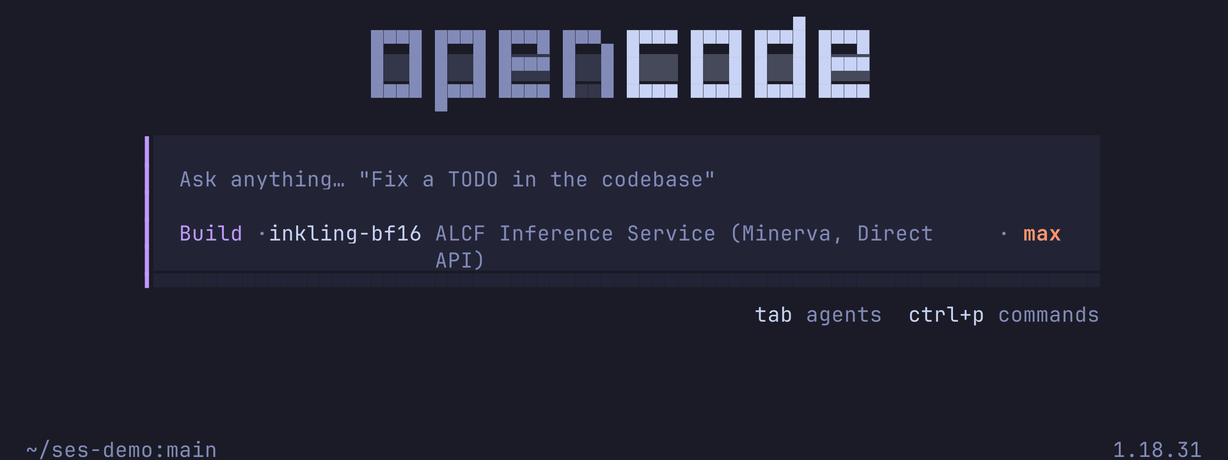
\includegraphics[width=0.80\textwidth]{opencode-shots/crop-a.png}
  \end{figure}
  \begin{itemize}
    \item Run \texttt{opencode} inside your project!
    \item \texttt{Ctrl+P} lists every command
  \end{itemize}
  \vspace{0.4em}
\end{frame}

\begin{frame}[fragile]{Talking to the Agent: \texttt{@}, \texttt{!}, and \texttt{/}}
  \begin{itemize}
    \item \texttt{@} adds a file or folder to the message by fuzzy search:
  \end{itemize}
  \begin{minted}[fontsize=\footnotesize]{text}
Refactor the error handling in @src/solve.py
Compare our output to @reference/README.md
  \end{minted}
  \begin{itemize}
    \item \texttt{!} runs a shell command and feeds the output back in:
  \end{itemize}
  \begin{minted}[fontsize=\footnotesize]{text}
!git log --oneline -5
  \end{minted}
  \begin{itemize}
    \item \texttt{/} runs an agent command.
      \begin{itemize}
        \item \texttt{/init} writes an \texttt{AGENTS.md} that it reuses on
          later turns
        \item Try \texttt{/models}, \texttt{/sessions}, and \texttt{/compact}!
      \end{itemize}
  \end{itemize}
\end{frame}

\begin{frame}{Watching the Agent Work}
  \begin{itemize}
    \item Your prompt, the model's reasoning, and every \textbf{tool call}
      show as a transcript in your terminal
    \item Here \texttt{Grep} found the file and \texttt{Read} opened it, so
      you can audit exactly what it saw
  \end{itemize}
  \vspace{0.4em}
  \begin{figure}
    \centering
    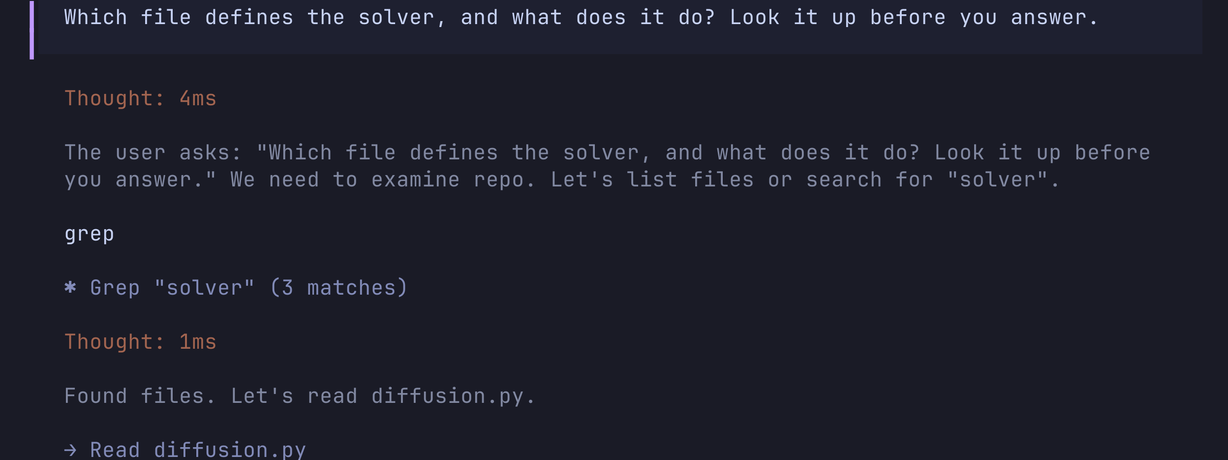
\includegraphics[width=0.82\textwidth]{opencode-shots/crop-b.png}
  \end{figure}
\end{frame}

\begin{frame}{Plan First, Then Build}
  \begin{itemize}
    \item \texttt{Tab} switches between the \textbf{Build} and \textbf{Plan}
      agents, the prompt box shows which is active
    \item \textbf{Plan} mode does its best to only analyze and propose changes
  \end{itemize}
  \vspace{0.4em}
  \begin{figure}
    \centering
    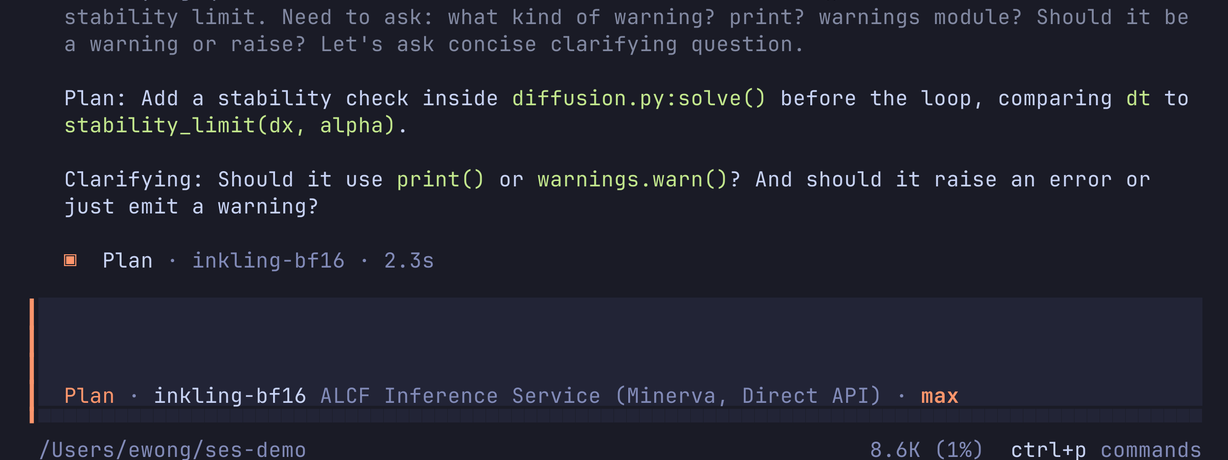
\includegraphics[width=0.80\textwidth]{opencode-shots/crop-c.png}
  \end{figure}
\end{frame}

\begin{frame}{Subagents and Orchestration}
  \begin{itemize}
    \item \textbf{Primary} agents are what you \texttt{Tab} between.
    \item \textbf{Subagents} are workers they delegate to, or that you call
      with \texttt{@explore}
    \item Built in: \texttt{general} (parallel units of work),
      \texttt{explore} (read-only code search), \texttt{scout} (upstream docs)
  \end{itemize}
  \vspace{0.4em}
  \begin{columns}[T]
    \begin{column}{0.48\textwidth}
      \centering
      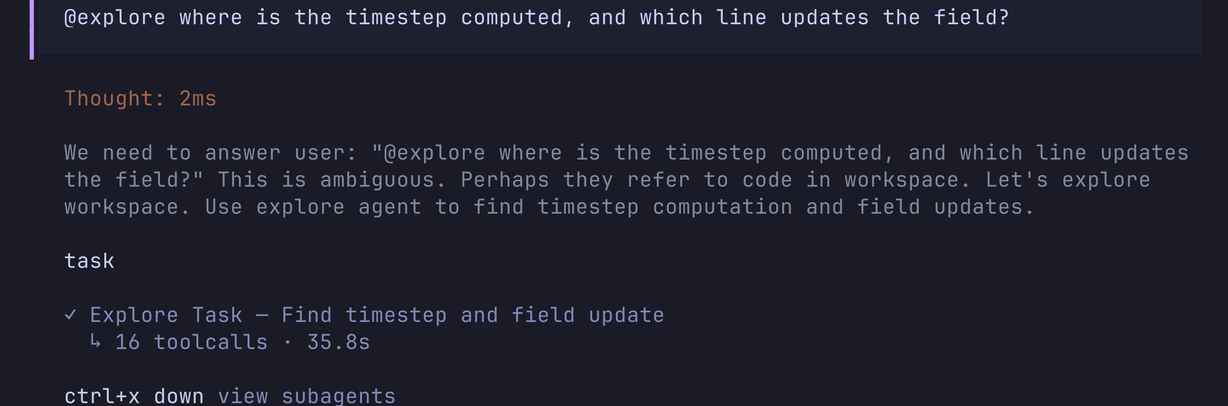
\includegraphics[width=\textwidth]{opencode-shots/crop-subagent.png}
    \end{column}
    \begin{column}{0.48\textwidth}
      \centering
      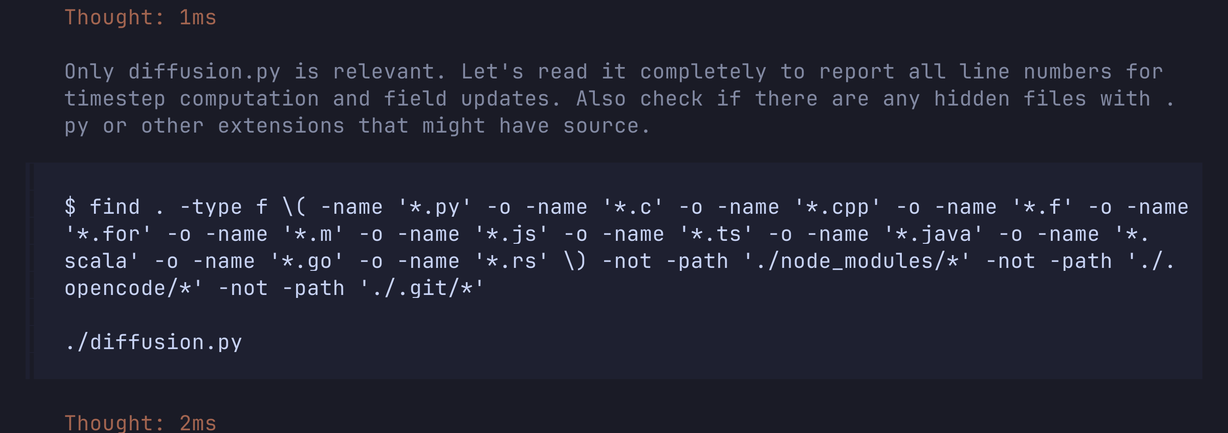
\includegraphics[width=\textwidth]{opencode-shots/crop-subagent-child.png}
    \end{column}
  \end{columns}
  \vspace{0.3em}
  \centering
  \footnotesize the delegate, and the worker's own session (\texttt{Ctrl+X down})
\end{frame}

\begin{frame}[fragile]{Permissions}
  \begin{itemize}
    \item Every tool is gated \texttt{allow}, \texttt{ask}, or \texttt{deny} ---
      \textbf{Plan} is just this, with edits and bash set to \texttt{ask}
  \end{itemize}
  \begin{minted}[fontsize=\footnotesize]{json}
{
  "permission": { "edit": "ask", "webfetch": "deny" },
  "agent": { "reviewer": { "permission": {
    "bash": { "*": "ask", "git diff": "allow" } } } }
}
  \end{minted}
  \begin{itemize}
    \item Bash rules take globs and the \textbf{last match wins}: put
      \texttt{"*": "ask"} before \texttt{"git diff": "allow"}
    \item \texttt{permission.task} gates which subagents an agent may call;
      \texttt{--auto} approves everything you did not deny
  \end{itemize}
\end{frame}

\begin{frame}{Review the Diff}
  \begin{itemize}
    \item Every edit displays as a \textbf{diff} with line numbers, just like
      in \texttt{git}
    \item Review the diff alongside summaries. Make incremental changes with
      each prompt, then test the code
  \end{itemize}
  \vspace{0.4em}
  \begin{figure}
    \centering
    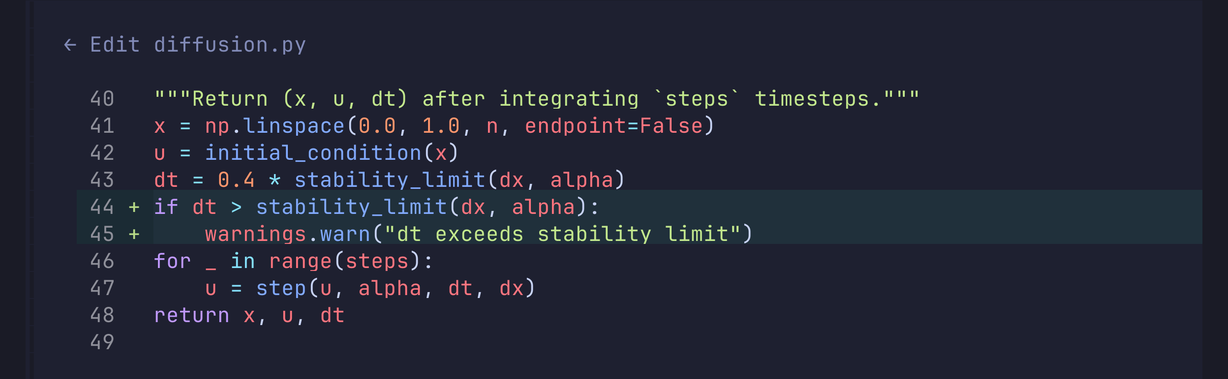
\includegraphics[width=0.85\textwidth]{opencode-shots/crop-d.png}
  \end{figure}
\end{frame}

\begin{frame}{Undo and Restore}
  \begin{itemize}
    \item \texttt{/undo} reverts the last change and hands your original
      prompt back so you can amend it\footnote{git stays your
      real undo button, though}
    \item \texttt{/redo} (or \texttt{Ctrl+X r}) re-runs it
  \end{itemize}
  \begin{figure}
    \centering
    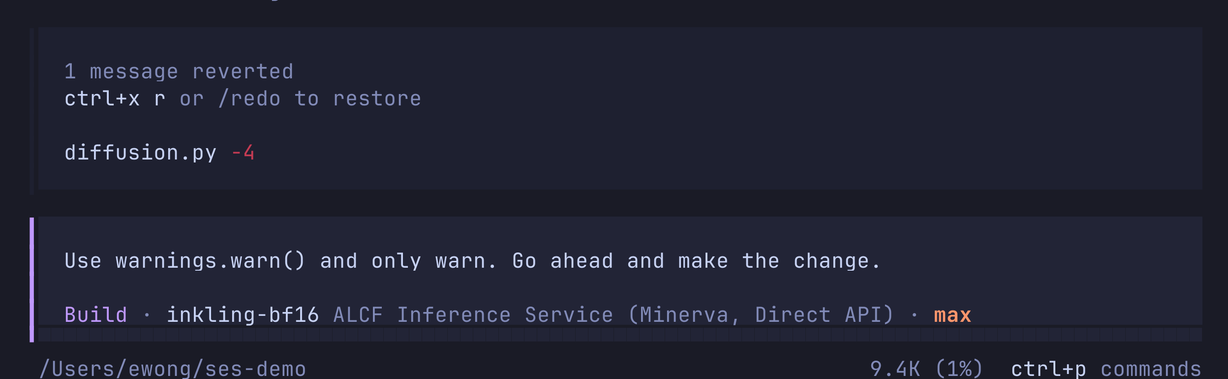
\includegraphics[width=0.85\textwidth]{opencode-shots/crop-e.png}
  \end{figure}
\end{frame}

\begin{frame}[fragile]{Sessions and Sharing}
  \begin{itemize}
    \item A \textbf{session} is one conversation
      \begin{itemize}
        \item \texttt{/sessions} switches between them
        \item \texttt{/new} starts a clean one
      \end{itemize}
    \item \texttt{/share} publishes the transcript and copies a link, which you
      can import with \texttt{opencode import}
      \begin{itemize}
        \item Note: share links are \textbf{public}
        \item A project config can set \texttt{"share": "disabled"} to prevent
          this
      \end{itemize}
    \item \texttt{--continue} and \texttt{--session} resume from the CLI
    \item \texttt{--fork} branches so the original stays intact
  \end{itemize}
\end{frame}

\section{Effective Vibecoding}

\begin{frame}{Iterate in Small Loops}
  \begin{itemize}
    \item \textbf{Plan before you build:} ask the agent to read the code and
      propose a plan first; review it, then let it code
    \item \textbf{One feature per prompt:} small steps, run the code after
      every change, commit after every success
    \item \textbf{Don't fight a confused agent:} if it spirals, restate the
      goal with clearer context, or start a fresh session instead of piling on
      corrections
    \item Git is your undo button; a clean history of small commits makes every
      agent edit cheap to review or revert
  \end{itemize}
  \vspace{0.8em}
  \centering
  \textit{Manage the agent like guiding a \emph{very} pedantic junior engineer!
  Small, well-defined tasks can be easily accomplished over broad, unscoped
  ideas.}
\end{frame}

\begin{frame}{Context is Everything}
  \begin{itemize}
    \item Keep an \textbf{instructions file} (\texttt{AGENTS.md},
      \texttt{CLAUDE.md}, \dots) at the repo root:
      project purpose, build/run/test commands, conventions, and
      no-go zones (\enquote*{never touch \texttt{src/legacy}})
    \item \textbf{Point, don't paste:} tell the agent which files matter
      and let it read/search the rest; pasted code goes stale
    \item \textbf{Fresh session per task:} long transcripts rot the
      model's working memory (the context window) and the agent's judgment
    \item Encode your \textbf{domain knowledge} explicitly: units, file
      formats, expected values, edge cases. The model cannot guess
      your physics.
  \end{itemize}
\end{frame}

\begin{frame}{Make Success Verifiable}
  \begin{itemize}
    \item Agents shine when \emph{correctness is checkable}; tests,
      linters, type checkers, a run script that prints a known result
    \item \textbf{Failing-test-first:} \enquote{write a test that captures the
      requirement, then make it pass}. Works extremely well for scientific
      codes
    \item Paste error messages back \emph{verbatim}; the agent can read
      tracebacks without needing to paraphrase
    \item For science: vetted outputs, sanity-limit checks, property tests.
      Verify figures against results you know.
  \end{itemize}
\end{frame}

\begin{frame}{Stay in Control}
  \begin{itemize}
    \item \textbf{Review the work!} Ultimately, you are responsible for what
      ships (papers, repos, production)
    \item Be cautious and \textbf{mandate human intervention} for destructive or
      far-reaching tasks; sandbox the agent when you can
    \item \textbf{Never paste tokens or credentials} into a prompt;
      keep secrets out of transcripts
    \item Models \textbf{hallucinate}: invented APIs, imaginary flags,
      plausible-but-wrong physics. Verify imports, citations, and
      values. Don't blindly trust the agent!!!
    \item Know when \emph{not} to vibe: unverifiable correctness-critical
      code, security-sensitive paths, etc.
  \end{itemize}
\end{frame}

\section{Crash Course}

\begin{frame}{Exercise: Vibecoded Monte Carlo $\pi$}
  \begin{columns}[T]
    \begin{column}{0.56\textwidth}
      \begin{itemize}
        \item Throw $N$ random darts at the unit square; the fraction $p$
          landing in the quarter circle estimates its area:
          \[
            \hat\pi = 4p, \qquad
            \sigma_{\hat\pi} = 4\sqrt{p(1-p)/N}
          \]
        \item Small enough to finish in one session, yet it has everything
          real science code has: numerics, an error bar, a known answer,
          and a figure
        \item Same loop every step: \textbf{prompt $\rightarrow$ code
          $\rightarrow$ \texttt{python pi\_mc.py} $\rightarrow$ look at the
          plot $\rightarrow$ refine}
        \item You are the architect; the agent is the executor;
          $\pi$ is the referee
      \end{itemize}
    \end{column}
    \begin{column}{0.40\textwidth}
      \centering
      \begin{tikzpicture}[scale=2.6]
        \fill[SESpanelLight] (0,0) rectangle (1,1);
        \fill[SESteal!25] (0,0) -- (1,0) arc[start angle=0, end angle=90, radius=1] -- cycle;
        \draw[SESgrey] (0,0) rectangle (1,1);
        \draw[SESink, thick] (1,0) arc[start angle=0, end angle=90, radius=1];
        \foreach \x/\y in {0.12/0.31,0.44/0.18,0.63/0.52,0.27/0.77,0.81/0.29,
                           0.35/0.46,0.55/0.71,0.18/0.58,0.72/0.12,0.49/0.38}
          \fill[SESteal] (\x,\y) circle (0.022);
        \foreach \x/\y in {0.91/0.71,0.78/0.88,0.95/0.44,0.66/0.93}
          \fill[orange!85!black] (\x,\y) circle (0.022);
        \node[below, font=\footnotesize, text=SESgrey] at (0.5,0)
          {$\hat\pi = 4 \times$ inside\,/\,all};
      \end{tikzpicture}
    \end{column}
  \end{columns}
\end{frame}

\begin{frame}[fragile]{Environment Setup}
  \begin{itemize}
    \item \textbf{Checklist:} \texttt{setup.sh} has already installed uv,
      OpenCode, and the Python environment, logged you in, and set up
      OpenCode for ALCF
  \end{itemize}
  \begin{minted}[fontsize=\footnotesize]{bash}
cd Service_Enabled_Science
./setup.sh                    # safe to re-run; sets up env + agents
source .venv/bin/activate     # numpy + matplotlib now on PATH

mkdir -p ~/pi-demo && cd ~/pi-demo
git init                      # your undo button
opencode                      # pick inkling-bf16 (Minerva)
  \end{minted}
  \begin{itemize}
    \item Use a new, empty directory so the agent can't find the
      reference \texttt{solution.py}
    \item The full prompt and the follow-ups are in
      \texttt{04\_Coding\_with\_Inference\_Service/PROMPT.md}
  \end{itemize}
\end{frame}

\begin{frame}[fragile]{Anatomy of a Good Prompt}
  \begin{columns}[T]
    \begin{column}{0.50\textwidth}
      \begin{minted}[fontsize=\tiny]{text}
Write a single Python script, pi_mc.py, that
estimates pi with Monte Carlo sampling and makes
a publication-quality figure of the result.

Environment:
- Use the `python` already on PATH (numpy +
  matplotlib). Do not pip install anything.
- Headless: savefig only, never plt.show().

The math:
- N uniform points, np.random.default_rng(seed),
  vectorized; pi_hat = 4p;
  stderr = 4*sqrt(p(1-p)/N).
- Print the estimate +/- stderr; fail if it is
  more than 3 stderr from math.pi.

The figure: (1) dartboard scatter, (2) running
estimate with a +/-2 sigma band on a log x-axis,
(3) log-log error vs. a sigma/sqrt(N) line.

Then run it twice, show me the output, and fix
any errors before you report back.
      \end{minted}
    \end{column}
    \begin{column}{0.46\textwidth}
      \begin{itemize}\small
        \item \textbf{Name the deliverable:} one file, one output
        \item \textbf{Pin the environment:} open models guess the
          environment wrong unless you tell them what's installed
        \item \textbf{Spell out the science:} formulas, units, and expected
          values; the model struggles with niche domain knowledge
        \item \textbf{Describe the figure panel by panel:}
          \enquote{make it pretty} gives a generic plot
        \item \textbf{Build in a check:} the $3\sigma$ assert and
          \enquote{run it} let the agent fix its own mistakes
      \end{itemize}
    \end{column}
  \end{columns}
\end{frame}

\begin{frame}{What Good Looks Like}
  \centering
  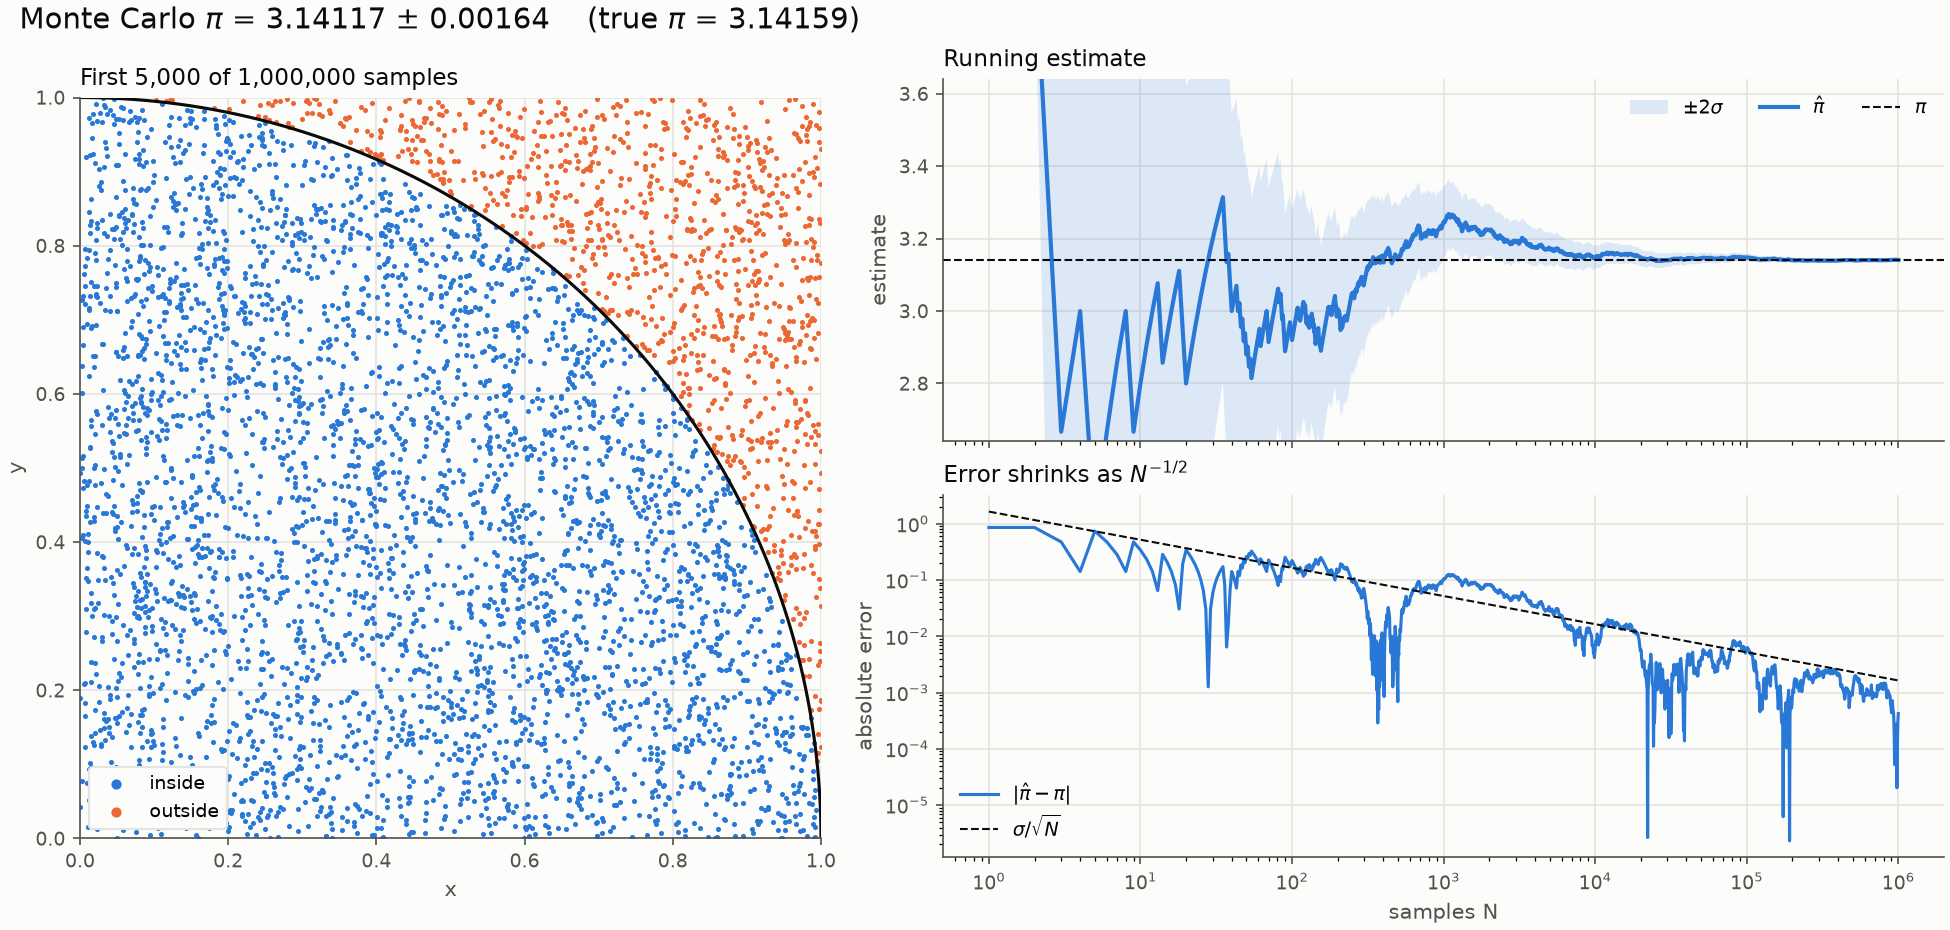
\includegraphics[height=0.60\textheight]{figures/pi_monte_carlo.png}\par
  \vspace{0.3em}
  \footnotesize\raggedright
  $10^6$ samples: $\hat\pi = 3.14117 \pm 0.00164$, which is $0.26\sigma$
  from $\pi$. The error follows the $N^{-1/2}$ line, so each additional
  digit of $\pi$ takes $100\times$ more samples.
\end{frame}

\begin{frame}{Check the Agent's Work, Then Push Further}
  \begin{columns}[T]
    \begin{column}{0.48\textwidth}
      \textbf{Verify}
      \begin{itemize}\small
        \item Run it yourself: $10^6$ samples should give an estimate
          within $\sim$0.003 of $\pi$
        \item Open the PNG: dots split at the arc, the estimate settles
          onto $\pi$, the error slope matches $N^{-1/2}$
        \item Read the diff: no Python loop over samples, no
          \texttt{plt.show()}, no \texttt{pip install}
        \item Commit once it works
      \end{itemize}
    \end{column}
    \begin{column}{0.48\textwidth}
      \textbf{Then, one prompt at a time}
      \begin{itemize}\small
        \item Run $K$ independent seeds: is their spread consistent with
          the standard error?
        \item Time $N = 10^5 \dots 10^8$ and report how runtime scales
        \item Add a \texttt{pytest} check against $\pi$ for several seeds
        \item Swap in a Sobol sequence (\texttt{scipy.stats.qmc}):
          how much faster does the error fall?
      \end{itemize}
    \end{column}
  \end{columns}
\end{frame}

\section{Going Further}

\begin{frame}{Skills, MCP, Plugins, and more}
  \begin{columns}[T]
    \begin{column}{0.52\textwidth}
      \begin{itemize}
        \item A \textbf{skill} is a folder with a \texttt{SKILL.md}: the agent
          sees only its \texttt{name}, \texttt{description}, and can call the
          \texttt{skill} tool when a task matches
        \item An \textbf{MCP server} adds server-provided tools, declared in
          \texttt{opencode.jsonc} under \texttt{mcp}
        \item \textbf{Plugins} are JS/TS that extends \texttt{opencode}'s own
          events, \texttt{alcf-ai-opencode-plugin} is one example
        \item Misc built-ins: \texttt{"lsp": true} gives the agent diagnostics,
          \texttt{"formatter": true} formats each edit
      \end{itemize}
    \end{column}
    \begin{column}{0.46\textwidth}
      \centering
      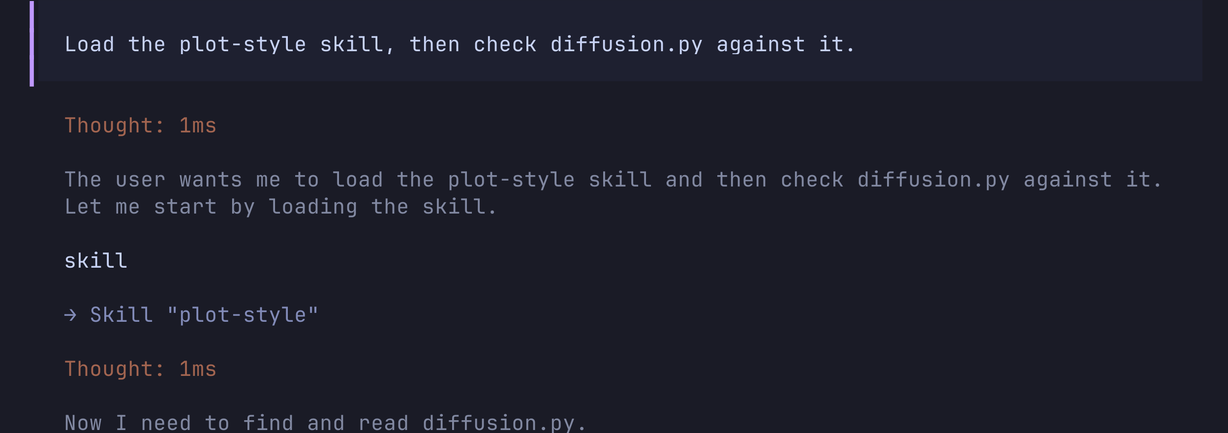
\includegraphics[width=\textwidth]{opencode-shots/crop-skill.png}
    \end{column}
  \end{columns}
  \vspace{0.4em}
  \footnotesize Next session uses Claude Code to demonstrate these
  capabilities! MCP in \texttt{.mcp.json}, skills in
  \texttt{\textasciitilde/.claude/skills/}.
\end{frame}

\appendix


\begin{frame}{References}
  \footnotesize
  \begin{itemize}
    \item ALCF Inference Endpoints docs (incl.\ \texttt{\#agents}):
      \url{https://docs.alcf.anl.gov/services/inference-endpoints}
    \item ALCF Inference Endpoints repo \& examples:
      \url{https://github.com/argonne-lcf/inference-endpoints}
    \item \texttt{alcf-ai} on PyPI:
      \url{https://pypi.org/project/alcf-ai/}
    \item Harness homepages: OpenCode \url{https://opencode.ai/}; Pi
      \url{https://pi.dev/}; Claude Code
      \url{https://code.claude.com/docs/en/quickstart}; Codex
      \url{https://learn.chatgpt.com/docs/codex/cli}
    \item Karpathy, A. (Feb 2025): \enquote{vibe coding} post on X
    \item Tanikanti et al., \textit{FIRST: Federated Inference Resource
      Scheduling Toolkit for Scientific AI Model Access}, SC Workshops '25.
      \url{https://doi.org/10.1145/3731599.3767346}
    \item Mailing list: \texttt{inference-service-notify} (
      \url{https://lists.alcf.anl.gov/mailman/listinfo/inference-service-notify})
  \end{itemize}
\end{frame}

\end{document}
